%implementing document formatting:
%page setup (page size, text size, page layout, chapters start on a new page).
%memoir is a form of book class that supports any kind of document.
\documentclass[fleqn,a4paper,12pt,twoside,openany,danish]{memoir}

%setting the header and footer in that order:
\setheadfoot{28pt}{28pt} %if any problems are encountered, try changing the latter 28pt with 1cm.

%setting language:
\RequirePackage[danish]{babel}

\usepackage{tocbibind}

%this package makes it possible to treat any element as a float,
%figures and tables are by default treated as floats.
%read http://en.wikibooks.org/wiki/LaTeX/Floats,_Figures_and_Captions to specify your float.
\usepackage{float}
\usepackage{wrapfig}
\usepackage{placeins}
\usepackage{tabu}

%this package makes it possible to make theorems and examples:
\usepackage{amsthm}
%setting the style of examples (parameters: plain, definition, remark):
%(definition is usually used for examples)
\theoremstyle{definition}
%the frist parameter is the syntax used in the document, the second is that which is printed in LaTex.
\newtheorem{example}{Eksempel}

%making it possible to use æ, ø and å:
\usepackage[utf8]{inputenc}
%helps with word division when using æ, ø and å, and makes it ps-font rather than bmp:
\usepackage[T1]{fontenc}

%package for implementation of graphic files:
\usepackage{graphicx}

\usepackage{multirow}

%package for subfigures
%\usepackage{graphicx}
%\usepackage{caption}


%package for captions
\usepackage[nooneline,labelfont=bf]{caption}
%\usepackage{subcaption}

%%package for implementation of math:
\usepackage{amsmath , amsfonts , amssymb, float}

%allowing use of color:
\usepackage{color}
%allowing use of more colors also in tables (see: http://en.wikibooks.org/wiki/LaTeX/Colors):
\usepackage[usenames,dvipsnames,svgnames,table]{xcolor}

%hyperlinks in the tabel of contents - comment this out before the report is printed.
\usepackage{hyperref}
\hypersetup{
%	bookmarks = true,  % Show 'bookmark'-frame in pdf.
	colorlinks = true, % True = colored links, False = framed links.
	citecolor = black,  % Link color for references.
	linkcolor = black,  % Link color in table of contents.
	urlcolor = black,   % Link color for extern URLs.
}

%makes it possible to refer to the name of a chapter rather than just the number.
\usepackage{nameref}

%package for the SI unit standard
\usepackage{siunitx}
\usepackage{units}

%package for writing program code in latex
\usepackage{listings}

\lstset{ 
language=C,               	 	% choose the language of the code
basicstyle=\footnotesize,       % the size of the fonts that are used for the code
numbers=left,                   % where to put the line-numbers
numberstyle=\footnotesize,      % the size of the fonts that are used for the line-numbers
stepnumber=1,                   % the step between two line-numbers. If it is 1 each line will be numbered
numbersep=5pt,                  % how far the line-numbers are from the code
backgroundcolor=\color{white},  % choose the background color. You must add \usepackage{color}
showspaces=false,               % show spaces adding particular underscores
showstringspaces=false,         % underline spaces within strings
showtabs=false,                 % show tabs within strings adding particular underscores
frame=single,           		% adds a frame around the code
tabsize=2,          			% sets default tabsize to 2 spaces
captionpos=b,           		% sets the caption-position to bottom
breaklines=true,       			% sets automatic line breaking
breakatwhitespace=false,    	% sets if automatic breaks should only happen at whitespace
escapeinside={\%*}{*)}          % if you want to add a comment within your code
}

%setting references (using numbers) and supporting i.a. Chicargo-style:
\usepackage{etex}
\usepackage{etoolbox}
\usepackage{keyval}
\usepackage{ifthen}
\usepackage{url}
\usepackage{csquotes}
\usepackage[backend=biber,url=true,doi=true,style=numeric, sorting=none]{biblatex}
\bibliography{bibliography/bibliography.bib}


%this package makes it possible include pdf pages in fx appendix;
%using  following syntax: \includepdf[pages={1}]{myfile.pdf}
\usepackage{pdfpages}

%%%MARGINER%%%
\setlrmarginsandblock{3.5cm}{2.5cm}{*}	% \setlrmarginsandblock{inner margin}{outer margin}{ratio}
\setulmarginsandblock{2.5cm}{3.0cm}{*}	% \setulmarginsandblock{top}{bottom}{ratio}
\checkandfixthelayout 			            % fixes stuff..

%%%%% Afsnitsformatering %%%%%%
\setlength{\parindent}{6mm}				% Stoerrelsen af indryk
\setlength{\parskip}{0mm}				% Afstand mellem afsnit ved 2xenter
\linespread{1,1}						% Linje afstand 

%Enables the use FiXme refferences. Syntax: \fxnote{...}
%With "final" in stead of "draft" an error will ocure for every FiXme
%under compilation.
\usepackage[footnote,draft,english,silent,nomargin]{fixme}

\addto\captionsdanish{% Replace "english" with the language you use
	\renewcommand{\contentsname}%
	{Indholdsfortegnelse}%
}

%%%CHAPTERLAYOUT%%%
%setting the color of the chapter number
\definecolor{numbercolor}{gray}{0.7}
%Downloaded chapter-setup:
\newif\ifchapternonum
\makechapterstyle{jenor}{
  \renewcommand\printchaptername{}
  \renewcommand\printchapternum{}
  \renewcommand\printchapternonum{\chapternonumtrue}
  \renewcommand\chaptitlefont{\fontfamily{pbk}\fontseries{db}\fontshape{n}\fontsize{25}{35}\selectfont\raggedleft}
  \renewcommand\chapnumfont{\fontfamily{pbk}\fontseries{m}\fontshape{n}\fontsize{1in}{0in}\selectfont\color{numbercolor}}
  \renewcommand\printchaptertitle[1]{%
    \noindent
    \ifchapternonum
    \begin{tabularx}{\textwidth}{X}
    {\let\\\newline\chaptitlefont ##1\par} 
    \end{tabularx}
    \par\vskip-2.5mm\hrule
    \else
    \begin{tabularx}{\textwidth}{Xl}
    {\parbox[b]{\linewidth}{\chaptitlefont ##1}} & \raisebox{-15pt}{\chapnumfont \thechapter}
    \end{tabularx}
    \par\vskip2mm\hrule
    \fi
  }
}
%setting chapter style:
\chapterstyle{jenor}

\makepagestyle{AAU}							% Definerer sidehoved og sidefod udseende frem til ...
\makepsmarks{AAU}{%
	\createmark{chapter}{left}{shownumber}{}{. \ }
	\createmark{section}{right}{shownumber}{}{. \ }
	\createplainmark{toc}{both}{\contentsname}
	\createplainmark{lof}{both}{\listfigurename}
	\createplainmark{lot}{both}{\listtablename}
	\createplainmark{bib}{both}{\bibname}
	\createplainmark{index}{both}{\indexname}
	\createplainmark{glossary}{both}{\glossaryname}
}
\nouppercaseheads											% Ingen Caps oenskes

\makeevenhead{AAU}{}{}{\leftmark}				% Definerer lige siders sidehoved (\makeevenhead{Navn}{Venstre}{Center}{Hoejre})
\makeoddhead{AAU}{\rightmark}{}{Aalborg Universitet}		% Definerer ulige siders sidehoved (\makeoddhead{Navn}{Venstre}{Center}{Hoejre})
\makeevenfoot{AAU}{\thepage}{}{}							% Definerer lige siders sidefod (\makeevenfoot{Navn}{Venstre}{Center}{Hoejre})
\makeoddfoot{AAU}{}{}{\thepage}								% Definerer ulige siders sidefod (\makeoddfoot{Navn}{Venstre}{Center}{Hoejre})
\makeheadrule{AAU}{\textwidth}{0.5pt}						% Tilfoejer en streg under sidehovedets indhold
\makefootrule{AAU}{\textwidth}{0.5pt}{1mm}					% Tilfoejer en streg under sidefodens indhold

\copypagestyle{AAUchap}{AAU}								% Sidehoved for kapitelsider defineres som standardsider, men med blank sidehoved
\makeoddhead{AAUchap}{}{}{}
\makeevenhead{AAUchap}{}{}{}
\makeheadrule{AAUchap}{\textwidth}{0pt}
\aliaspagestyle{chapter}{AAUchap}							% Den ny style vaelges til at gaelde for chapters
% ... her

\pagestyle{AAU}												% Valg af sidehoved og sidefod

\usepackage{textpos}

%depth of numbered headlines (part/chapter/section/subsection):
\setsecnumdepth{subsection}
\maxsecnumdepth{subsection}
%depth of the table of contents:
\settocdepth{subsection}

% Makes sure LaTeX does not stretch the text at page break:
\raggedbottom

%Figure references:
\newcommand{\figref}[1]{figur \ref{#1}}

%Figure references after full stop/period:
\newcommand{\Figref}[1]{Figur \ref{#1}}

%Table references:
\newcommand{\tabref}[1]{tabel \ref{#1}}

%Table references after full stop/period:
\newcommand{\Tabref}[1]{Tabel \ref{#1}}

%Section references:
\newcommand{\secref}[1]{afsnit \ref{#1} på side \pageref{#1}}

%Section references:
\newcommand{\Secref}[1]{Afsnit \ref{#1} på side \pageref{#1}}

%Appendix references:
\newcommand{\appref}[1]{appendiks \ref{#1} på side \pageref{#1}}

%Appendix references:
\newcommand{\Appref}[1]{Appendiks \ref{#1} på side \pageref{#1}}

%chapter references: 
\newcommand{\chapref}[1]{kapitel \ref{#1} på side \pageref{#1}}

%chapter references: 
\newcommand{\Chapref}[1]{Kapitel \ref{#1} på side \pageref{#1}}

%Units:
%\newcommand{\unit}[1]{&& \left[\si{#1}\right]}

%Text:
\newcommand{\tx}[1]{\text{#1}}

%Equation references:
%1 equation:
\renewcommand{\eqref}[1]{ligning (\ref{#1})}
%2 equations:
%\newcommand{\eqrefTwo}[2]{ligning (\ref{#1})} and \textbf{(\ref{#2})}
%%3 equations:
%\newcommand{\eqrefThree}[3]{ligning (\ref{#1})}, \textbf{(\ref{#2})} and \textbf{(\ref{#3})}
%%4 equations:
%\newcommand{\eqrefFour}[4]{ligning (\ref{#1})}, \textbf{(\ref{#2})}, \textbf{(\ref{#3})} and \textbf{(\ref{#4})}
%%5 equations:
%\newcommand{\eqrefFive}[5]{ligning (\ref{#1})}, \textbf{(\ref{#2})}, \textbf{(\ref{#3})}, \textbf{(\ref{#4})} and \textbf{(\ref{#5})}
%%5 equations:
%\newcommand{\eqrefSix}[6]{ligning (\ref{#1})}, \textbf{(\ref{#2})}, \textbf{(\ref{#3})}, \textbf{(\ref{#4})}, \textbf{(\ref{#5})} and \textbf{(\ref{#6})}
%%5 equations:
%\newcommand{\eqrefSeven}[7]{ligning (\ref{#1})}, \textbf{(\ref{#2})}, \textbf{(\ref{#3})}, \textbf{(\ref{#4})}, \textbf{(\ref{#5})}, \textbf{(\ref{#6})} and \textbf{(\ref{#7})}
%
%%Equation references after full stop/period:
%%1 equation:
%\newcommand{\Eqref}[1]{Ligning (\ref{#1})}
%%2 equations:
%\newcommand{\EqrefTwo}[2]{Ligning (\ref{#1})} and \textbf{(\ref{#2})}
%%3 equations:
%\newcommand{\EqrefThree}[3]{Ligning (\ref{#1})}, \textbf{(\ref{#2})} and \textbf{(\ref{#3})}
%%4 equations:
%\newcommand{\EqrefFour}[4]{Ligning (\ref{#1})}, \textbf{(\ref{#2})}, \textbf{(\ref{#3})} and \textbf{(\ref{#4})}
%%5 equations:
%\newcommand{\EqrefFive}[5]{Ligning (\ref{#1})}, \textbf{(\ref{#2})}, \textbf{(\ref{#3})}, \textbf{(\ref{#4})} and \textbf{(\ref{#5})}
%%5 equations:
%\newcommand{\EqrefSix}[6]{Ligning (\ref{#1})}, \textbf{(\ref{#2})}, \textbf{(\ref{#3})}, \textbf{(\ref{#4})}, \textbf{(\ref{#5})} and \textbf{(\ref{#6})}
%%5 equations:
%\newcommand{\EqrefSeven}[7]{Ligning (\ref{#1})}, \textbf{(\ref{#2})}, \textbf{(\ref{#3})}, \textbf{(\ref{#4})}, \textbf{(\ref{#5})}, \textbf{(\ref{#6})} and \textbf{(\ref{#7})}
\begin{document}

%||||||||||||||||||||||||||||||||||||||||||||||||||||||||||||||||
%|||||||				Example Inputs					 ||||||||
%||||||||||||||||||||||||||||||||||||||||||||||||||||||||||||||||
%|||||||												 ||||||||
%	\section{Figure Sample}

\begin{figure}[H]
	\centering
	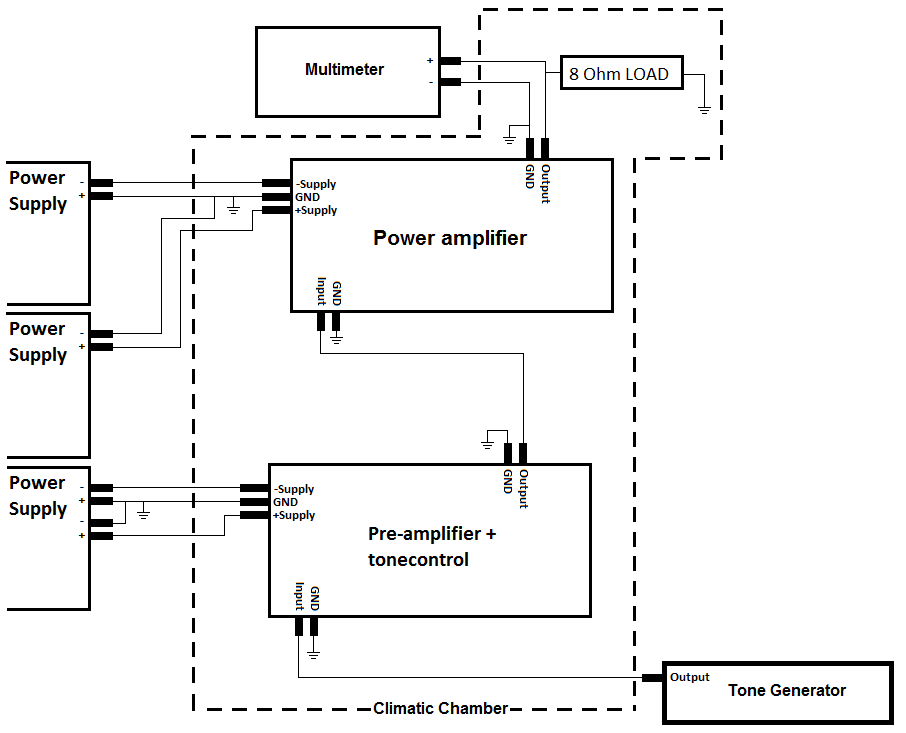
\includegraphics[scale=.8]{figures/filename}
	\flushleft 
	\caption{CAPTION\fxnote{Remember source}}
	\label{LABEL}
	\flushleft
	\textit{SOURCE}
\end{figure}

%--------- NOTES ------------------------------------------------------
%Fxnotes wont compile properly inside the figure, only in the caption.
%Filetype can be specified but isn't needed.

\noindent
\figref{LABEL}\\

\noindent
\Figref{LABEL}

\vspace{.5cm}
%Do not use \vspace{length} or \hspace{length} unless exceedingly necessary.

%--------- BIBLIOGRAPHY REF EKSAMPLE -----------------------------------
This reference only represents this line since it is before the punctuation mark\cite{YDing}. This next reference however represents the entire section. That is all of the preceding sentences in the entire section. This is due to the fact that it is now after the punctuation mark in the end of the section (this is not used in the middle of a section!).\cite{YDing}
%>>>>>>>>>>>>>>>PLEASE ALSO READ THE NOTE IN myBib.bib<<<<<<<<<<<<<<<<<<
\pagebreak	%||||||||
%	\section{Table Sample}

\begin{table}[H]
\caption{This Is a Table\label{LABEL}}
\begin{tabular}{|l|p{5cm}|l|l|l|}
  \hline
  \textbf{No.}&\textbf{Description}&\textbf{Min}&\textbf{Max}&\textbf{Requirements}\\
  \hline
  1 & Some Text & Some Text & Some Text & Some Text\\
    &           &           &           & Some More Text\\
    &           &           &           & Text Text\\
    &           &           &           & Text Text Text\\
  \hline
  2 & Some Text & Some Text & Some Text & Some Text\\
  \hline
  3 & 	By specifying the width of a column (|p\{5cm\}|) the cells
  		in that column will will not exceed	the specified width    %Enter is used only for clarity and will not affect the compiled output.
  		but instead expand downward.
  		
  		        & Some Text & Some Text & Some Text\\
  \hline
  4 & Some Text & Some Text & Some Text & Some Text\\
  \hline
  \multicolumn{2}{|l|}{Some Text} 	&	\multicolumn{3}{l|}{Some Text}\\
  \hline
  \multicolumn{2}{|l|}{Text Text} 	&	\multicolumn{3}{l|}{Text = Text}\\
  \multicolumn{2}{|l|}{}			&	\multicolumn{3}{l|}{Text = Text}\\
  \multicolumn{2}{|l|}{}			&	\multicolumn{3}{l|}{Text = Text}\\
  \multicolumn{2}{|l|}{}			&	\multicolumn{3}{l|}{Text = Text}\\
  \multicolumn{2}{|l|}{}			&	\multicolumn{3}{l|}{Text = Text}\\
  \hline
  \multicolumn{2}{|l|}{Some Text} 	&	\multicolumn{3}{l|}{Teeeexxtt}\\
  \multicolumn{2}{|l|}{}			&	\multicolumn{3}{l|}{\LaTeX}\\
  \hline      
\end{tabular}
\end{table}

\noindent
\tabref{LABEL}\\

\noindent
\Tabref{LABEL}

\pagebreak	%||||||||
%	\section{Equation Sample}

Ohms Law:
\begin{flalign}
  U &= I \times R \unit{\volt}
  \label{eq1}
\end{flalign}
%
Some explanation:
\begin{flalign}
  [Equation] &= [Number] \unit{Unit}
  \label{eq2}
\end{flalign}
%
Some explanation:
\begin{flalign}
  [Equation] &= [Number] \unit{Unit}
  \label{eq3}
\end{flalign}
%
Some explanation:
\begin{flalign}
  [Equation] &= [Number] \unit{Unit}
  \label{eq4}
\end{flalign}
%
Some explanation:
\begin{flalign}
  [Short Equation] &= [Number] \unit{Unit}
  \label{eq5}\\ %<-------------------------------------------------| Remember linebreak AFTER
  [Somewhat Longer Equation] &= [Number] \unit{Unit} %             | label when writing multiple
  \label{eq6}\\ %<-------------------------------------------------| equations.
  [Somewhat Quite a Lot Longer Equation] &= [Number] \unit{Unit}
  \label{eq7}
\end{flalign}
%
%
\eqref{eq1}\\
%
\eqrefTwo{eq1}{eq2}\\
%
\eqrefThree{eq1}{eq2}{eq3}\\
%
\eqrefFour{eq1}{eq2}{eq3}{eq4}\\
%
\eqrefFive{eq1}{eq2}{eq3}{eq4}{eq5}\\
%
\eqrefSix{eq1}{eq2}{eq3}{eq4}{eq5}{eq6}\\
%
\eqrefSeven{eq1}{eq2}{eq3}{eq4}{eq5}{eq6}{eq7}\\
%
\Eqref{eq1}\\
%
\EqrefTwo{eq1}{eq2}\\
%
\EqrefThree{eq1}{eq2}{eq3}\\
%
\EqrefFour{eq1}{eq2}{eq3}{eq4}\\
%
\EqrefFive{eq1}{eq2}{eq3}{eq4}{eq5}\\
%
\EqrefSix{eq1}{eq2}{eq3}{eq4}{eq5}{eq6}\\
%
\EqrefSeven{eq1}{eq2}{eq3}{eq4}{eq5}{eq6}{eq7}
%
\pagebreak	%||||||||
%|||||||												 ||||||||
%||||||||||||||||||||||||||||||||||||||||||||||||||||||||||||||||
%||||||||||||||||||||||||||||||||||||||||||||||||||||||||||||||||


%implementing front page:
\clearpage
\thispagestyle{empty}

\begin{figure}[H]
	\raggedleft
		
\includegraphics[width=0.2\textwidth]{figures/aaulogo-da.png}
\end{figure} 
\vspace*{\fill} 
\begin{center}	
\begin{Huge}
\textbf{Prædiktiv model til kapacitetsudnyttelse}\\
\vspace{5 mm}
P$5$ Semestersprojekt - Efteråret $2016$\\
\vspace{3 mm}
\end{Huge}
{\Large Gruppe $5405$}
\end{center}
\vspace*{\fill}

\begin{center}
\line(1,0){400}
\end{center}

%clears one or two pages to make the document start on right hand side:
\cleardoublepage

%numbers the pages with Roman numeral - starts from "i":
\frontmatter

%implementing title sheet:
%\begin{document} 
\thispagestyle{empty}
%\begin{titlepage}
\begin{nopagebreak}
	{\samepage 
		
		\begin{tabular}{r}
			\parbox{\textwidth}{  \raisebox{11mm}{
\includegraphics[height=2cm]{figures/aaulogo-da.png}}
				\hfill \hspace{2cm} \parbox{8cm}{\begin{tabular}{l} %4.90
						{\small \textbf{\textcolor{MidnightBlue}{{$5$. Semester}}}}\\
						{\small \textbf{\textcolor{MidnightBlue}{School of Medicine and Health}}}\\
						%{\small \textbf{\textcolor{MidnightBlue}{}}}\\ 
						{\small \textbf{\textcolor{MidnightBlue}{Sundhedsteknologi}}}\\
						{\small \textcolor{NavyBlue}{Fredrik Bajers Vej $7$A}} \\
						{\small \textcolor{NavyBlue}{$9220$ Aalborg}} \\
						%{\small \textcolor{NavyBlue}{\emph{http://www.smh.aau.dk/}}}
			\end{tabular}}}
		\end{tabular}
		
		\begin{tabular}{cc}
			\parbox{7cm}{
				\begin{description}

%\item {Titel:}
%
%Prædiktiv model til kapacitetsudnyttelse\\

\item {Tema:} 

\small{
Klinisk teknologi
}

\end{description}

\parbox{8cm}{

\begin{description}
\item {Projektperiode:}\\
   P$5$, Efteråret $2016$\\
   
\item {Projektgruppe:}\\
  $5405$\\
  
\item {Medvirkende:}\\
Linette Helena Poulsen\\
Maria Kaalund Kroustrup\\
Nirusha Jeevanadan \\
Rolf Oberlin Hansen\\
Sageevan Sayananthan \\
Sebastian Munk \\

\hspace{2cm}
\item {Vejleder:}\\
Hovedevejleder: Pia B. Elberg \\
Kliniske vejleder: Sten Rasmussen \\
Klinisk bivejleder: Christian Kruse. \\  
\end{description}

}
\begin{description}
\item {Sider: XX}
\item {Appendikser: XX}
\item {Afsluttet:}
\end{description}
\vfill } &
\parbox{7cm}{
  \vspace{.15cm}
  \hfill 
  \begin{tabular}{l}
  {Synopsis:}\bigskip \\
  \fbox{
    \parbox{6.5cm}{\bigskip
     {\vfill{\small Overlæge Sten Rasmussen udtaler, at omfanget af kapacitetsmangel på ortopædkirurgisk afdeling på Aalborg Universitetshospital opleves stigende og tiltagende. Hertil forekommer der i år $2017$ en ny budgetaftale, der omhandler hurtigere udredning. Dette forventes at kunne skabe udfordringer for patientplanlægningen og kapacitetsudnyttelsen. Ubalance i kapacitetsudnyttelsen kan medvirke til komplikationer ift. arbejdsvilkår og patientsikkerhed. Herved kan en effektivisering af planlægningen medvirke til at opretholde en balance i kapacitetsudnyttelsen. En mulig løsning til dette kan være anvendelse af prædiktiv modellering til estimering af elektive patienters indlæggelsesvarighed. Det kan konkluderes, at en prædiktiv model kan anvendes til at estimere indlæggelsesvarigheden. Det er på baggrund af denne projektrapport ikke muligt at vurdere præcisionen af denne model, hvorfor yderligere studier er påkrævet.
     \bigskip}}
     }}
   \end{tabular}}
\end{tabular}} \vspace{1.3cm}
\raggedleft
\textit{\tiny Offentliggørelse af rapportens indhold, med kildeangivelse, må kun ske efter aftale med forfatterne.}\nopagebreak
\\
\end{nopagebreak}
%\end{titlepage}
%\end{document}
 \cleardoublepage

% FORORD OG LÆSEVEJLEDNING
\chapter*{Forord og læsevejledning}

\section*{Forord}
Dette projekt er udarbejdet af gruppe $16$gr$5405$, $5$. semesters studerende på ingeniøruddannelsen sundhedsteknologi på Aalborg Universitet. Projektet er udarbejdet i perioden $2$. september til $19$. december år $2016$. Projektforslaget er stillet af Sten Rasmussen, overlæge på ortopædkirurgisk afdeling på Aalborg Universitetshospital, og omhandler prædiktiv modellering til forudsigelse af indlæggelsesvarigheden for patienter mhp. at effektivisere planlægningen. 


Vi vil gerne takke hovedevejleder Pia B. Elberg, kliniske vejleder Sten Rasmussen samt kliniske bi-vejleder Christian Kruse for vejledning og feedback gennem hele projektperioden. Derudover vil vi give en særlig tak til ortopædkirurgisk afdeling på Aalborg Universitetshospital for samarbejdet. 


\section*{Læsevejledning}
Rapporten er inddelt i fem kapitler. Det første kapitel indeholder projektets indledning samt den initierende problemstilling, der ligger til grund for problemanalysen, som fremgår af andet kapitel. Metoden beskrives i tredje kapitel. Fjerde kapitel analyserer implementeringen af en prædiktiv model på ortopædkirurgisk afdeling ift. forudsigelse af indlæggelsesvarighed for patienter mhp. planlægning af disse. Det fjerde kapitel er syntese, der indeholder en diskussion, konklusion samt perspektivering af projektet. Kapitlerne efterfølges af bibliografi samt bilag. 


Til håndtering af kilder anvendes Vancouver-metoden. De anvendte kilder nummereres i kantede parenteser. Er referencen placeret efter et punktum i en sætning, tilhører den hele afsnittet. Er referencen placeret før et punktum, tilhører den sætningen. Er der placeret flere referencer efter hinanden, betyder dette, at der er anvendt flere referencer til den pågældende sætning eller afsnit. Referencer til bilag er ligeledes indsat i kantede parenteser og er placeret efter samme metode som kilder. 

Forkortelser er skrevet ud ved første anvendelse, hvorefter forkortelsen er skrevet i parentes. Denne forkortelse anvendes herefter fremadrettet i rapporten. 


Rapporten er udarbejdet i \LaTeX, herudover anvendes MATLAB $2016$b til databehandling samt visualisering af grafer. 
 \cleardoublepage

%the '*' allows the tableofcontents be excepted from the actual table of contents.
\tableofcontents*
\cleardoublepage

%numbers the pages with Arabic numeral - starts from 1.
\mainmatter

%---------------------------INPUTS-------------------------------


% INDLEDNING

\chapter{Indledning}


Flere danske hospitalsafdelinger oplever i perioder at have flere patienter end der er kapacitet til, i form af mangel på sengepladser, personale eller rum\cite{Company2013}. Overskridelsen af kapaciteten resulterer bl.a. i, at personalet får mindre tid pr. indlagt patient, hvilket kan medføre gener for både personalet og patienter.\cite{Kjeldsen2015} I budgetfordelingen for Aalborg Universitetshospital i år 2017 indgår det, at ventetiden på en operation for elektive patienter skal reduceres fra 57 dage til 50 dage\cite{Budget2016}. Dette forventes at medføre, at det daglige antal elektive patienter, der indlægges, vil skabe en reducering i antallet af ledige sengepladser til akutte patienter. 

Et estimat fra 2016 indikerer, at procentdelen af danskere over 65 år vil stige fra $29~\%$ til $34~\%$ og dermed også antallet af patienter\cite{RegionNord2016}. En stigning i antallet af patienter vil i takt med kortere ventetid på behandling skabe et aktuelt problem ift. planlægning af indlæggelser samt kapacitetudnyttelse på ortopædkirurgisk afdeling. Ifølge en undersøgelse fra Dansk Sygeplejeråd, mener hver anden regionalt ansat sygeplejerske på tværs af regionerne, at den travle arbejdsdag påvirker patientsikkerheden\cite{Kjeldsen2015}. Foruden personalets øgede risiko for at begå fejl ift. behandlingen af patienter, kan der ligeledes opstå en sundhedsrisiko ved kapacitetsmangel. Manglen på fysisk kapacitet kan give anledning til at overflytte patienter til uhensigtsmæssige områder som f.eks. hosptialsgange\cite{Madsen2014}. Dermed er der opstået et aktuelt problem som vedrører kapacitetsmangel, og konsekvenserne af dette problem bør undersøges nærmere. Ved at udnytte kapaciteten på afdelingen opnås der mere sundhed for pengene\cite{Company2013}. På baggrund af dette opstilles følgende initierende problem:

\textit{Hvordan påvirkes ortopædkirurgisk afdeling på Aalborg Universitetshospital af ændringerne vedrørende kapacitetsudnyttelse og hvor udbredte er belægningsrelaterede problemer på afdelingen?}





% Der er i dag overbelægning på flere afdelinger på de danske hospitaler, hvoraf nogle afdelingerne berøres i hele og flere måneder ad gangen. \cite{2015} Overbelægning resulterer i, at sundhedspersonalet får mindre tid pr. indlagt patient. Ifølge en undersøgelse fra Dansk Sygeplejeråd, mener hver anden regionalt ansat sygeplejerske på tværs af regionerne, at den travle arbejdsdag går ud over patienternes sikkerhed \cite{Kjeldsen2015}. Et studie påviser, at ved blot én ekstra indlagt patient pr. sygeplejerske øges mortalitetsraten med $7~\%$ indenfor en indlæggelse på 30 dage \fxnote{Har stadig lidt svært ved om man kan forstå sætningen på den rigtige måde.} \cite{Aiken2014}. 

% Foruden sundhedspersonalets øgede risiko for at begå fejl ift. behandlingen af patienter, er der ligeledes en sikkerhedsrisiko forbundet ved overbelægning på hospitalerne. De ekstra patienter, der ligger på stuerne, gangene og vaskerummene, pga. overbelægning, er en større udfordring ved evakuering under brand. Pladsmangel, som medfører, at patienterne opholder sig i vaskerummene og på gangene, bevirker desuden til, at patienterne oplever et skærpet privatliv. \cite{Madsen2014}

% Aalborg universitetshospital har i et tidligere projekt indsamlet data fra $1.000$ hospitalsindlæggelser. Disse data inkluderer blodprøveanalyser og knoglescanninger (DXA), hvilket formodes at kunne anvendes til udvikling af en prædiktiv model, der kan estimere indlæggelsesvarigheden blandt patienter. Denne rapport vil på baggrund af dette undersøge, hvorvidt det er muligt at forudsige indlæggelsesvarigheden ved brug af machine learning. \fxnote{mangler stadig noget om begrundelsen for valg af machine learning}



% \section{Initierende problemstilling} \fxnote{Dette er ikke den endelige problemstilling}
% Hvordan påvirkes personalet og patienterne af overbelægning på hospitaler, og hvilke konsekvenser har overbelægning i forhold til sikkerheden på afdelingerne?
% Hvilke typer af machine learning findes der, samt hvor benyttes det i dag?



% PROBLEMANALYSE
\input{contents/bProblemanalyse/A_ChapProblemanalyse.tex}
\input{contents/bProblemanalyse/bStress.tex}
\input{contents/bProblemanalyse/C_Skader.tex}
\input{contents/bProblemanalyse/okonomi.tex}
\input{contents/bProblemanalyse/xAfgraensning_problemformulering.tex}



% KRAVSPECIFIKATION
\input{contents/dSystemspecifikation/a_ChapKrav.tex}
\input{contents/dSystemspecifikation/b_Kravspecifikation.tex}


% SYSTEMDESIGN for hardware
\input{contents/eHardwareDesign/a_ChapHardwareDesign.tex}
\input{contents/eHardwareDesign/MotorOgHjul.tex}
\input{contents/eHardwareDesign/Navigation.tex}
\input{contents/eHardwareDesign/Computer.tex}


% SYSTEMDESIGN FOR SOFTWARE
\input{contents/fSoftwareDesign/a_ChapSoftwareDesign.tex}
\input{contents/fSoftwareDesign/c_Aktuatorer.tex}
\input{contents/fSoftwareDesign/e_UltraSoft.tex}
\input{contents/fSoftwareDesign/f_FarveSoft.tex}
\input{contents/fSoftwareDesign/g_Accelerometer.tex}
\input{contents/fSoftwareDesign/h_Fjernbetjening.tex}
\input{contents/fSoftwareDesign/m_Mainrutine.tex}

% SOFTWARE & HARDWARE DESIGN OG IMPLEMENTERING AF KOMMUNIKATIONSFORMER
%\input{contents/yTing_Vi_Maaske_Kan_Bruge_Senere/Kommunikationsformer.tex}

%% TEKNISK ANALYSE		*** skal være design ***
%\input{contents/cTekniskAnalyse/a_Chap_TekniskAnalyse.tex}
%%\input{contents/cTekniskAnalyse/bFunktionelleKrav.tex}
%\input{contents/cTekniskAnalyse/sensorerrrr.tex}
%\input{contents/cTekniskAnalyse/xTraadLoes.tex}
%\input{contents/cTekniskAnalyse/motor.tex}
%\input{contents/cTekniskAnalyse/omniwheels.tex}
%\input{contents/cTekniskAnalyse/ev3mindstorm.tex}
%%\input{contents/cTekniskAnalyse/UART_komunnikation.tex}
%\input{contents/cTekniskAnalyse/xBygningskrav.tex}
%\input{contents/cTekniskAnalyse/xAfgraensning.tex}


% IMPLEMENTERING
\input{contents/gImplementering/a_Chap_Implementering.tex}
\input{contents/gImplementering/xNedskaleredeKrav.tex}
\input{contents/gImplementering/xLedning.tex}
\input{contents/gImplementering/xMotorstyring.tex}
\input{contents/gImplementering/xArduinoTilPSoC.tex}
\input{contents/gImplementering/xFarvesensor.tex}
\input{contents/gImplementering/xUltralydssensor.tex}
\input{contents/gImplementering/xLineFollowing.tex}
\input{contents/gImplementering/xJoystickTing.tex}
\input{contents/gImplementering/xSamletSystem.tex}

% TEST
\input{contents/hTest/a_Chap_Test.tex}

% AFRUNDING
\input{contents/iDetDetAfsluttendeHalloej/aDiskussion.tex}
\input{contents/iDetDetAfsluttendeHalloej/bKonklusion.tex}
\input{contents/iDetDetAfsluttendeHalloej/cPerspektivering.tex}


\urlstyle{same}

\printbibliography
\cleardoublepage

% BILAG
\begin{appendices}
\input{contents/sAppendix/xBygningskrav.tex}
\end{appendices}

\end{document}